\input{preambuloSimple.tex}

%----------------------------------------------------------------------------------------
%	TÍTULO Y DATOS DEL ALUMNO
%----------------------------------------------------------------------------------------

\title{	
\normalfont \normalsize 
\textsc{{\bf Ingeniería de Servidores (2014-2015)} \\ Grado en Ingeniería Informática \\ Universidad de Granada} \\ [25pt] % Your university, school and/or department name(s)
\horrule{0.5pt} \\[0.4cm] % Thin top horizontal rule
\huge Memoria Práctica 1 \\ % The assignment title
\horrule{2pt} \\[0.5cm] % Thick bottom horizontal rule
}

\author{José Arcos Aneas} % Nombre y apellidos

\date{\normalsize\today} % Incluye la fecha actual

%----------------------------------------------------------------------------------------
% DOCUMENTO
%----------------------------------------------------------------------------------------

\begin{document}

\maketitle % Muestra el Título

\newpage %inserta un salto de página

\tableofcontents % para generar el índice de contenidos

\listoffigures


\newpage
%----------------------------------------------------------------------------------------
%	Cuesti´on 1
%----------------------------------------------------------------------------------------

\section{¿Qué modos y tipos de virtualización existen?}

Podríamos distinguir tres tipos de virtualización.

Virtualización completa.
	Donde la máquina virtual simula un hardware para permitir un sistema operativo "huesped" sin modificar, para efectuar de forma aislada. Este fue el primero en 1966  y es el predecesor de la familia de máquinas virtuales de IBM.
	
Virtualización parcial. "Addres Space Virtualization". La máquina virtual simula multiples instancias, de gran parte pero no todo, del entono suyacente del comaparti recursos, pero no permite instancias separadas de sistemas operativos "huésped". Aunque es vista como dentro de una categoria de maquina virtual, historicamente fue un importante acercamiento, y lo usaron en sistemas com oCTSS, el experimento IBM M44/44X.

Virtualización de sistema operativo.
	Esta vitualización mejora el rendimiento, gestión y eficiencia. En la base reside un SO (Sistema Operativo) anfitrión estándar, a continuación encontramos la capa de virtualización. con un sistema de archivos y una capa de abstracción de servivicio de kernel que garantice el aislamiento y seguridad de los recursos entre los distintos contenedores. La capa de virtualización hace que cada uno de los contenedores aparezca como servidor autónomo.
Máquina vrtual: Lo entenderemos como un sistema de cirtualización, habitualmente llamado "virtualizacion de servidores"	, es un software que lo que pretende es simular una computadora para ejecutar en ella programas como si fuera una máquina real.

	Respecto a los " modos ", la virtualización se hace desde un SO hasta otro, los diferentes modos que se pueden conseguir son:
	
	- Virtualización por hardware: extensiones introducidas en la arquitectura del x86 para facilitar las tareas la aquitectura. En esta nueva arquitectura se le introduce un anillo interior o ring-1 que sea el que un hypervisor o Virtual Machine Monitor usará para aislar las capas superiores de software de las operaciones de virtualización.
	
	- Virtualización de almacenamiento: Se refiere al proceso de abstraer el almacenamiento lógico del fisico. Los recursos de almacenamiento fisicos son agregados al "almacén de almacenamiento (strong pool),  del cual es creado el almacenamiento lógico.
	
	-Particionamiento: División de un solo recurso, como el espacio de disco o el achacho de banda de una red en un número mas pequeño y con recursos del mismo tipo que son más fáciles de utilizar. En almacenamiento real se le llama "zoning".
	
	- Máquina virtual: Todas las instancias dependen del mismo hardware y dispositivos físicos, pero casisiempre trabajan como modelos totalmente independientes.
	
	- Hypervisor de almacenamiento: En este pack portatil de gestion centralizada, utilizado pora mejorear el valor combinado de los sistemas de disco de alamcenamiento multiples, incluyendo los modelos diferentes e incomplatibles, completando sus capacidades individuales con el aprovisionamiento etendido, la réplica y l aaceleración del rendimiento del servicio. 



\section{Muestre los precios y características de varios proveedores de VPS (Virtual Private Server) y compare con el precio de servidores dedicados (administrados y no administrados) .}
\url{http://www.arsys.es/servidores/vps?gclid=CJy5y_u1_boCFfMctAodimIAYg/}
\begin{figure}[H]
\begin{center}
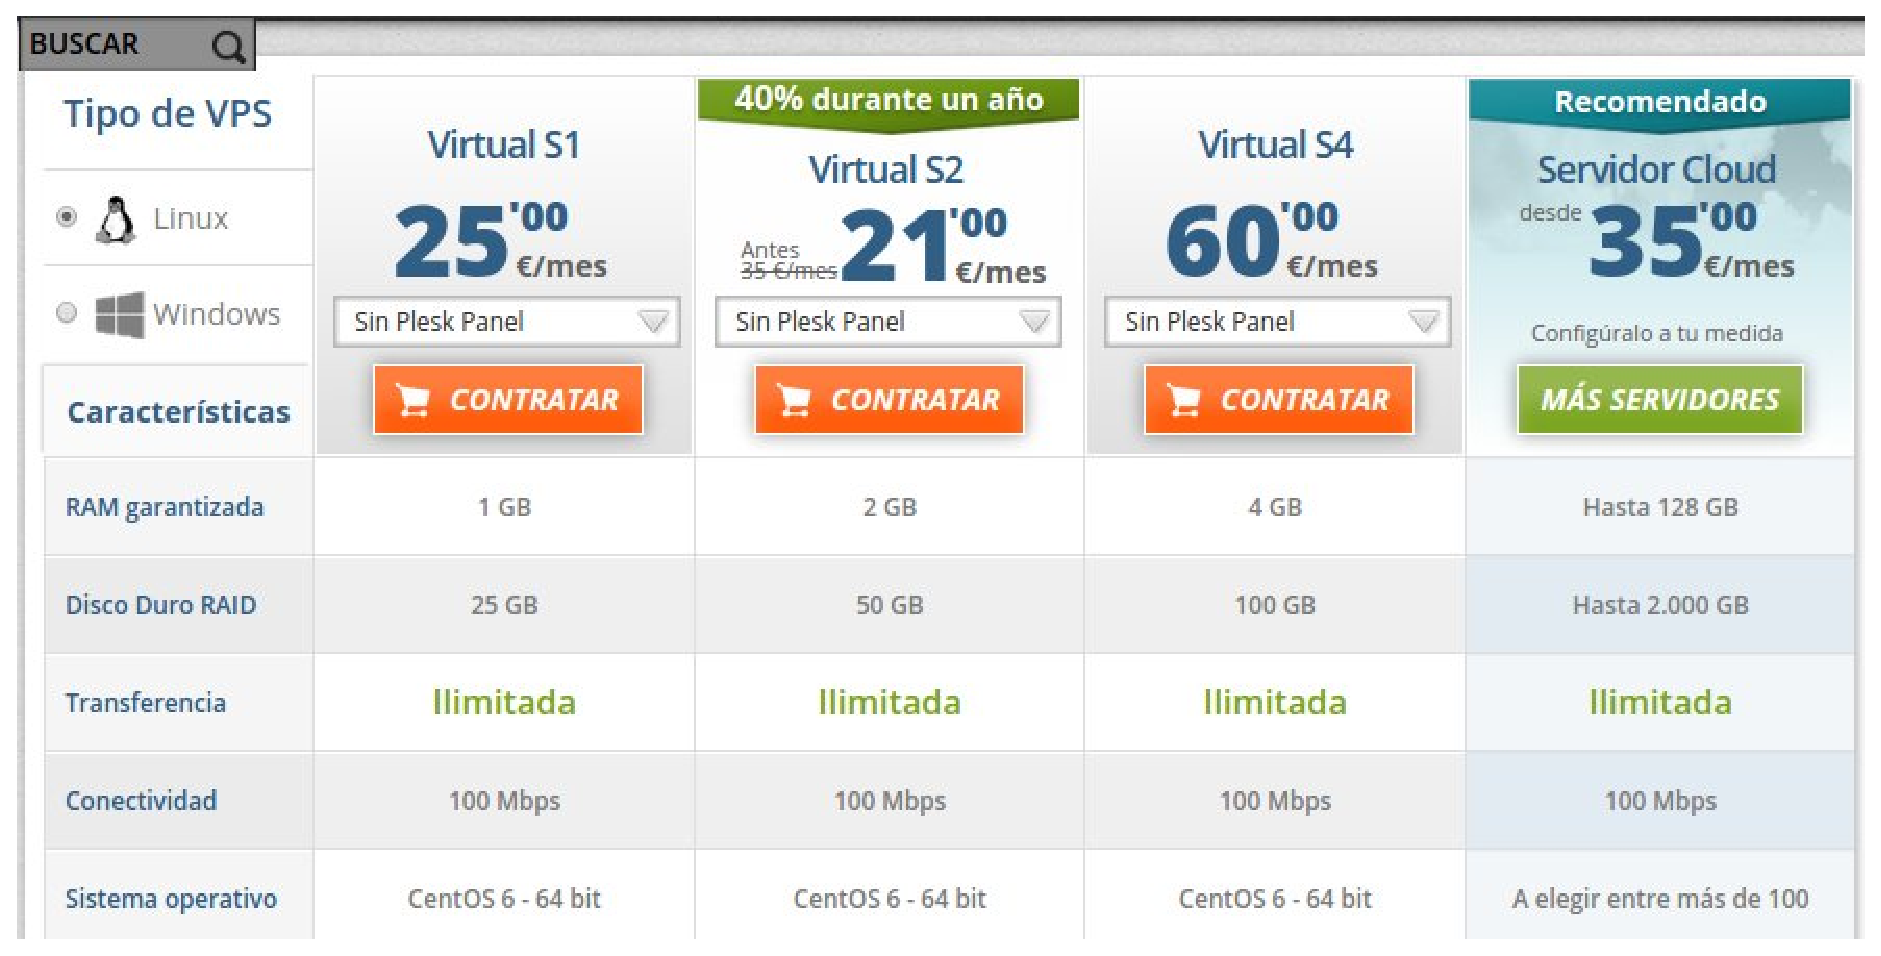
\includegraphics[scale=0.4]{imagenes/cuestion2-1.eps}
\caption{ Arsys vps linux.}
\end{center}
\end{figure}

\begin{figure}[H]
\begin{center}
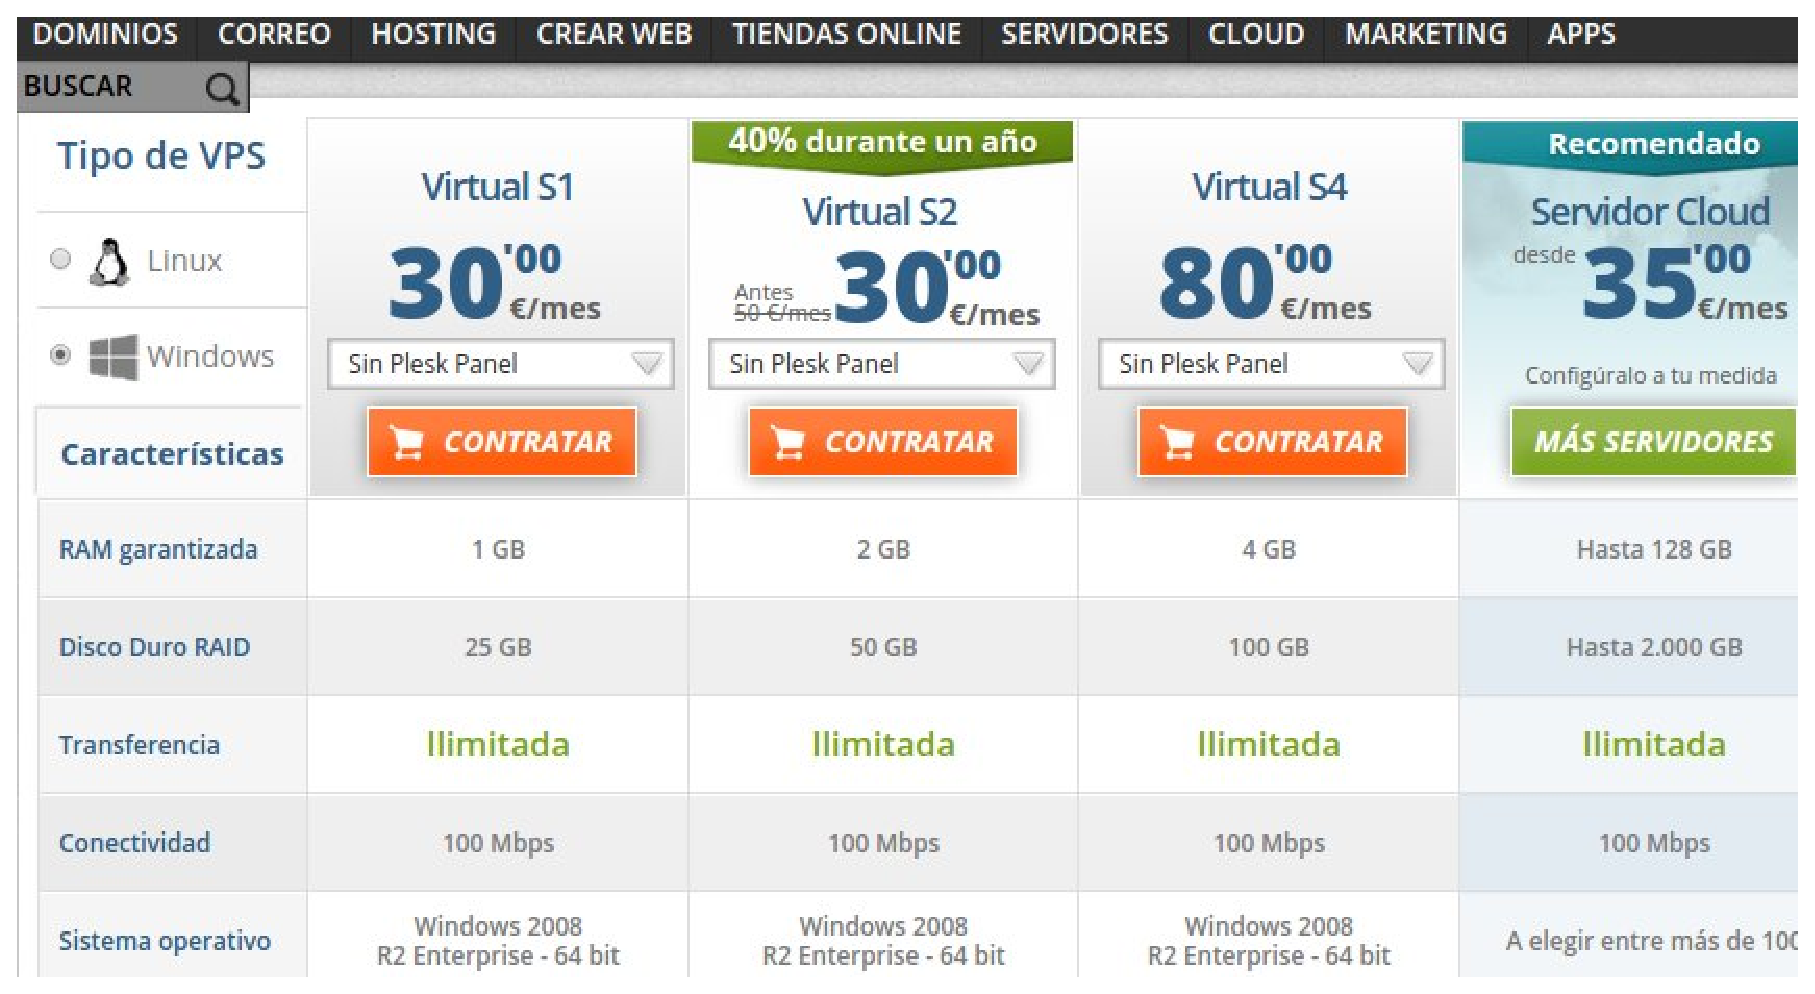
\includegraphics[scale=0.4]{imagenes/cuestion2-2.eps}
\caption{ Arsys vps windows.}
\end{center}
\end{figure}


\textbf{RedCoruna}
\url{http://www.redcoruna.com/hosting-vps.html}

Empresa RedCodura según he podido comprobar comercializa solo productos con software unix. 
\begin{figure}[H]
\begin{center}
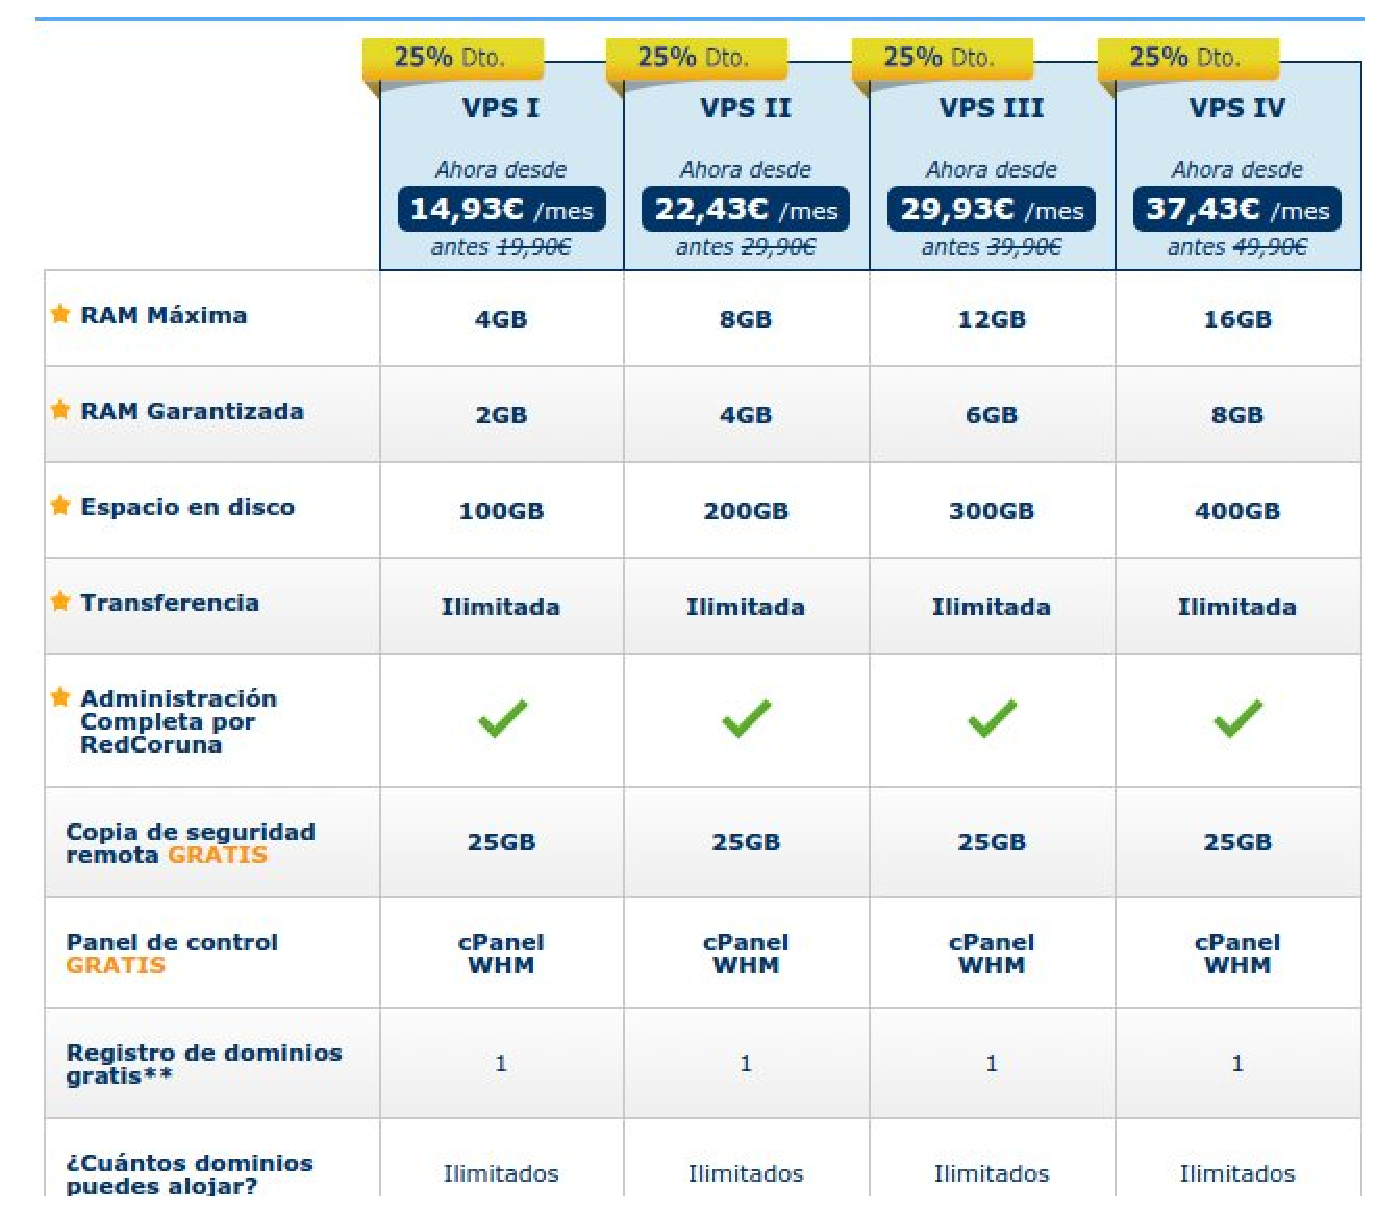
\includegraphics[scale=0.4]{imagenes/cuestion2-3.eps}
\caption{ RedCodura vps unix.}
\end{center}
\end{figure}


\textbf{Dinahosting}

\url{https://dinahosting.com/vps}



Solo usa Unix también.

\begin{figure}[H]
\begin{center}
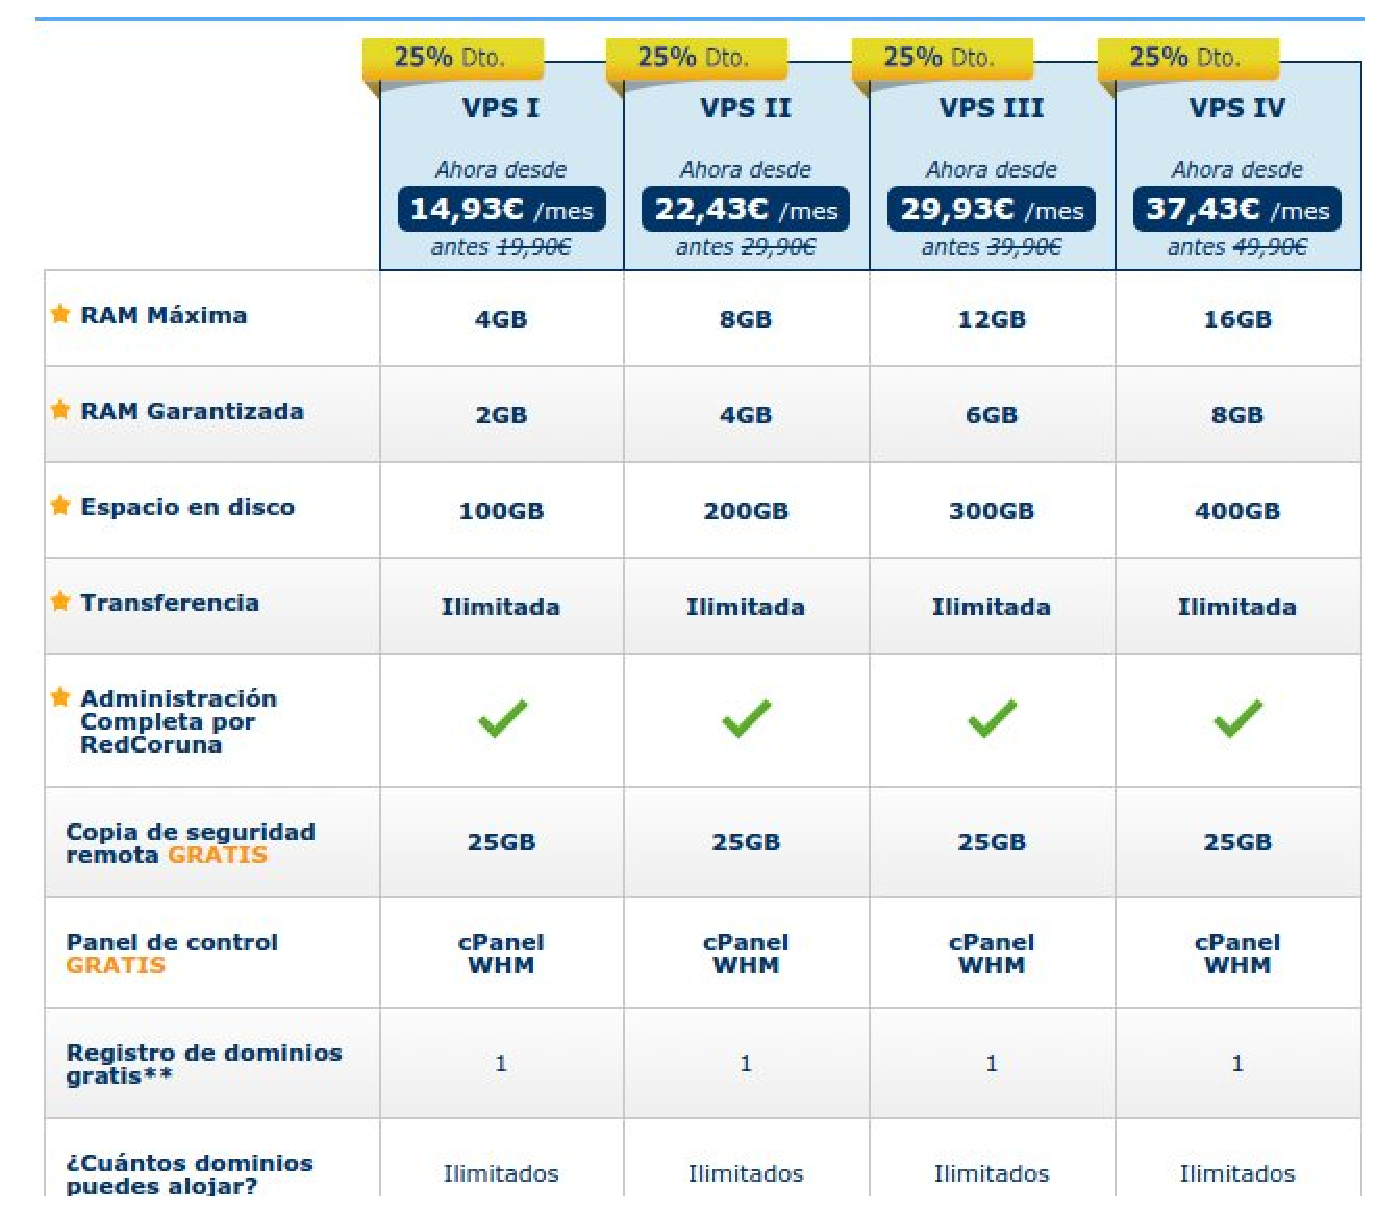
\includegraphics[scale=0.4]{imagenes/cuestion2-3.eps}
\caption{ Dinahosting vps Unix.}
\end{center}
\end{figure}

\textbf{Hostalia}
\url{http://www.hostalia.com/vps/}

Comercializa tanto con software de Unix como de Windows, aunque cabe destacar que la versión de Windows en bastante mas cara.
 
\begin{figure}[H]
\begin{center}
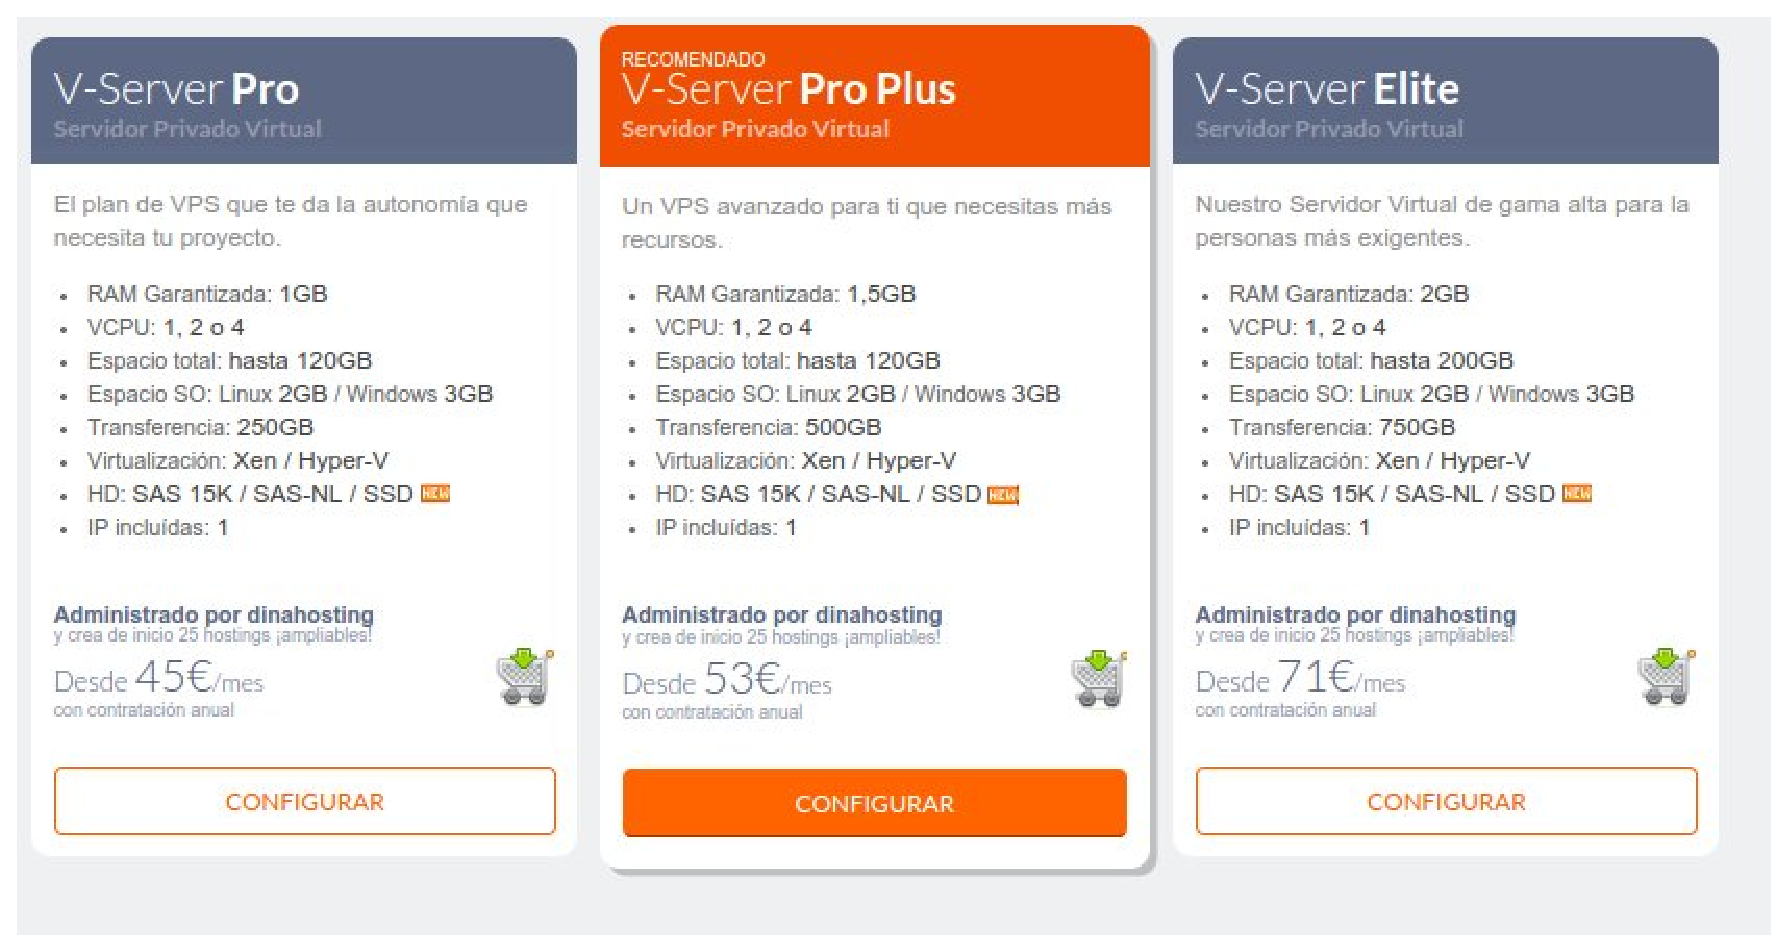
\includegraphics[scale=0.4]{imagenes/cuestion2-4.eps}
\caption{ "Hostalia" vps Unix y Windows.}
\end{center}
\end{figure}


%----------------------------------------------------------------------------------------
%	Cuesti´on 1
%----------------------------------------------------------------------------------------

\section{ ¿Qué otros software de vitualización, además de VMWARE y VBOX, hay? }
\begin{itemize}
\item \textit{OpenVZ} -> openvz.org/Main.Page
\item \textit{VirtualPC} -> wwww.microsoft.com/es-es/download/details.aspx?id=4580

\item \textit{linux-kvm.org/page/Main-Page}

\end{itemize}


\section{ Enumere algunas de las innovaciones de Windows 2012 respecto a 2008 R2. ¿ Es posible instalar Windows 2012 sin entorno gráfico?  }

No presentan innovaciones directa e inmediatas salvo la manejabilidad. No es posible instalarla pero una vez instalado es posible quitar el entorno gráfico. Esto suele hacerse para mejorar las prestaciones del servidor.


\section{¿Qué empresa hay detrás de Ubuntu?}
\footnote{http://www.canonical.com/}
Canonical, empresa británica propiedad de Mark Shuttleworth.

\subsection{¿Qué otros productos/servicios  ofrece?}

Se financia con servicions vinculados al sistema operativo, además también vende soporte técnico.



\subsection{¿Qué es MAAS?}

Es una herramienta de configuración, apoya el depliegue de infracestructuras comoOpenShack, Hadoop,CloudStack, LoadBalanced Web y clound Foundry. También gestiona servidores como un recurso similar a la nube.

\section{¿Qué relación tiene CentOS con RetHat  con fedora?}
\footnote{https://www.redhat.com/es/global/spain}
\footnote{https://getfedora.org/}

La página web de \textit{RetHat} mencionada anteriormente, dedica una página entera a la relación que existen entre estas dos plataformas. \footnote{https://www.redhat.com/es/technologies/linux-platforms/articles/relationship-between-fedora-and-rhel}
CentOS es una bifurcación a nivel binario de la districuvion de RetHat Enterprise Linus RHELL, a àrtir del código liberado por RetHat.

CentOs tambien utiliza la oden yum para bajar e instalar actualizaciones también utilizada en Fedora.


\section{Indique que otros SO se utilizan y el porcentaje de uso.}

Fedora, OpenSUSE, FreeBSD, Debian, RetHat. No he encontrado información sobre el porcentaje de uso de cada uno de estos SO.

Para ver el porcentaje de uso no he encontrado una página en concreto donde aparezca un analisis fiable, en cambio, si he podido encontrar un analisis comparativo , de cierta calidad, donde se analizan los porcentajes de uso de los diferentes sistemas operativos para servidores web.\footnote{ "Web Technologies Statistics and Trends". W3Techs. December 2013.}.

En la Wikipedia \footnote{http://en.wikipedia.org/wiki/Usage\_share\_of\_operating\_systems} podemos encontrar un análisis comparativo del uso de los diferentes sistemas operativos, Destacamos la siguiente tabla. Donde podemos encontrar el porcentaje de uso de cada sistema operativos en servidores de web públicos
\begin{figure}[H]
\begin{center}
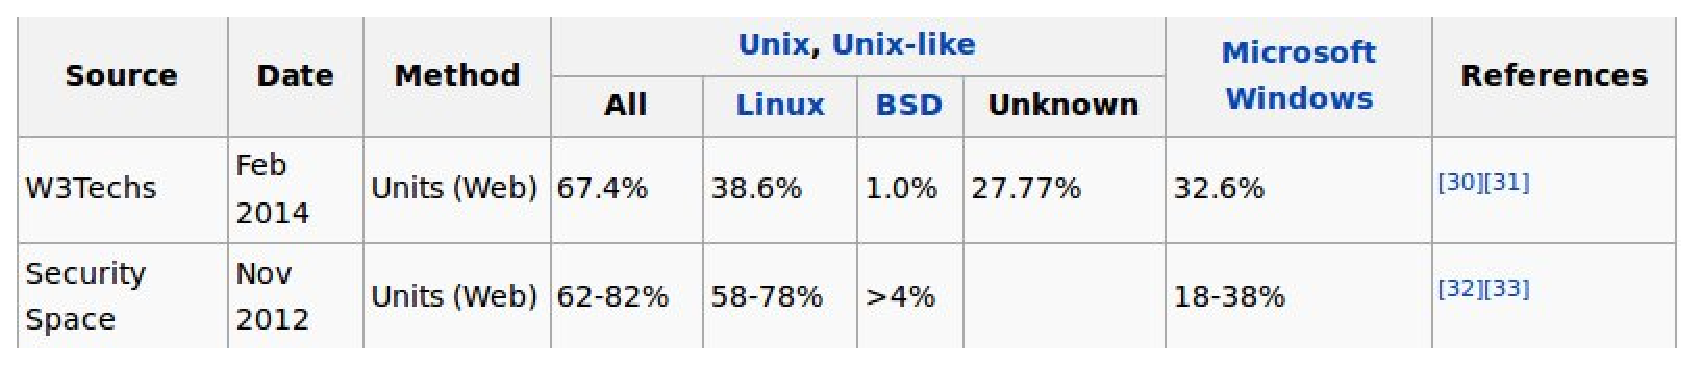
\includegraphics[scale=0.4]{imagenes/cuestion7.eps}
\caption{ Tabla extraída de la Wikipedia.}
\end{center}
\end{figure}
En la imagen anterior es posible obsevar el porcentaje de uso de los diferentes sistemas operativos en el caso de servidores web.
\section{¿De qué es el acrónimo de RAID?}
\footnote{http://es.wikipedia.org/wiki/RAID}
Proviene del inglés "Redundant Array of Independent Disk" originalmente "Redundant Array Inexpensive Disks", hace referencia a un sistema de almacenamiento de datos que usa multiples unidades de almacenamiento de datos entre las que distribuye o replican los datos.

\subsection{¿Qué tipos de RAID hay?}
Existen los niveles estandar (raid0, raid1,..., raid6) raid anidados y raid propietarios.

\subsection{¿Qué diferencia hay entre RAID mediante SW y mediante HW?}

Hice la prueba y la diferencia fue que por software no puede hacer que el RAID sea el disco de arranque.


\section{¿Qué es un LVM?}
LVM hace referencia a una forma de asignar espacio de forma mas eficiente que de las formas tradicionales (particinado). En particular puede concatenar, dividir, combinar particiones, incluso de distintos discos, en otras virtuales mas grandes.

\subsection{¿Qué ventajas tiene para un servidor de gama baja?}

Permite simular mas memoria.
\subsection{Si va a tener un servidor web,¿le daria un tamaño pequeño o grande a /var?}
Poca, para un servidro web no hace falta mucha. Aún asi, se podria crear un LVM y concatenarlo con otro disco, para si, por ejemplo se llena el disco asociado a el para otorgarle mas espacio.


\section{¿Debemos cifrar tambien el volumńe que contiene el espacio para SWAD?}

No, porque al ser un área de intercambio de archivos no tendrá sentido y se ralentiza el proceso.

\subsection{¿y el volumen en el que montaremos /boot?}

Depende, hay versiones de linux que no son capaces de arrancar una particion cifrada.

\section{¿Qué otro tipo de usos de una partición le permite configurar el asistente de instalación ?}

Te permite configurarla como lógica y principal.

\subsection{¿Qué diferencia principal hay entre ext4 y ext2?}

Ext2 y ext3 no soportan Link2SD.
\section{Muestre cómo ha quedado el disco particionado una vez el sistema está instalado. }

\begin{figure}[H]
\begin{center}
\includegraphics[scale=0.3]{imagenes/cuestion12-1.eps}
\caption{Imagen del lvm.}
\end{center}
\end{figure}

\begin{figure}[H]
\begin{center}
\includegraphics[scale=0.3]{imagenes/cuestion12-2.eps}
\caption{ Imagen del disco una vez particionado.}
\end{center}
\end{figure}

\section{¿Cómo ha hecho el disco2 " arrancable "?}

Con el comando grub -install se utiliza para configurar el grup de arranque. 

	"grub -install -boot -directory=/arraq"
	
\subsection{¿Qué hace el comando grub -install ?}

Su uso es indicarle al MBR si el grub se movio, la nueva estara donde este la seccion de arranque. Con el comando anterior MBR accdera a arranq/grub.

\subsection{¿Qué hace el comando dd?}
El comando "dd" (duplicate-disk) se usa para transferencia de archivos/directorios a otros archivos/directorios.

Se usa para crear imagenes .iso desde disco de arranque.
Tambien se usa para crear discos "arrancables" o "booteables" :

dd if=origen of=destino

\section{¿Qué diferencia hay entre Standard y Datacenter?}

La versión Datacenter, que incluye en su licenciamiento la capaciadad de albrgar dentro de HyperV una cantidad ilimitada de equipos virtuales. Para esquemas físicos o de baja virtualizacion, la version Standard permite el uso de 2 equipos virtuales destro de la misma licencia. Lo mejor de todo esto es que ambas versiones, Standard y Datacenter son idénticas en funcionalidades y prestaciones.


\footnote{ 
http://www.internetya.co/windows-server-2012-ediciones-datacenter-y-standard/}
\footnote{http://horacioag.wordpress.com/2012/11/07/diferencias-entre-la-version-standard-y-la-version-datacenter-de-windows-server-2012/}

\section{Continúe usted con el proceso de definición de RAID1 para los discos de 50MiB que ha creado. Muestre el proceso con capturas de pantalla.}
Hemos seguido estrictamente las instrucciones para crear un disco espejo en Windows. Básicamente son
los siguientes pasos:
\begin{itemize}
	\item 1. Elegimos crear un nuevo volumen reflejado.
\begin{figure}[H]
\begin{center}
\includegraphics[scale=0.4]{imagenes/cuestion15-1.eps}
\caption{Imagen del paso 1.}
\end{center}
\end{figure}
	\item 2. En la pantalla que nos aparece seleccionamos los discos que utilizaremos y el espacio.
	
\begin{figure}[H]
\begin{center}
\includegraphics[scale=0.4]{imagenes/cuestion15-2.eps}
\caption{Imagen del paso 2.}
\end{center}
\end{figure}
	\item 3. Elegimos la configuración (NTFS, tamaño predeterminado, Volumen Reflejado de
nombre).
\begin{figure}[H]
\begin{center}
\includegraphics[scale=0.4]{imagenes/cuestion15-3.eps}
\caption{Imagen del paso 3.}
\end{center}
\end{figure}
	\item 4. Confirmamos nuestra elección.
\begin{figure}[H]
\begin{center}
\includegraphics[scale=0.4]{imagenes/cuestion15-4.eps}
\caption{Imagen del paso 4.}
\end{center}
\end{figure}
	\item 5. El estado final de nuestros discos es esté.
\begin{figure}[H]
\begin{center}
\includegraphics[scale=0.4]{imagenes/cuestion15-5.eps}
\caption{Imagen del paso 5.}
\end{center}
\end{figure}
\end{itemize}

\section{¿Qué opciones establecen una red local con la máquina anfitriona ?}
Hay que primero cerrar la máquina.

Acceder a la pestaña Virtual Machine Setting, en la pestaña "Hardware".
Debe estar activo una opción en "Network connectin", estará establecida como NAT. Esta debemos dejarla asi. Esta hacen que comparta la misma IP's que el huésped.
	
Debemos agregar otro dispositivo. Opcion Network Adapter Host-only.
	Ya al inicial la maquina dispondremos de conexion a internet que estara conectada en erd con el host.
\subsection{¿ Con qué opción podemos compartir la conexión a Internet?}
Para esto usarémos \textit{NAT}, con lo que tanto anfitrión como huésped tendrán la misma dirección IP.
\section{¿Cómo podemos ver que ambas máquinas estan conectadas a la misma red local?}
\footnote{http://norfipc.com/redes/usar-comando-ping.html}
Uso del comando \textbf{ping} : \textit{ping -c 1 (numero de paquetes) x.x.x.x -> (direccion/nombre)}

Esta orden envia un numero de paquetes a un sistema que se identifica por su IP o nombre. Si recibimos respuesta de los paquetes significará que el sistema esta conectada.


\end{document}